% 75-25(75쪽) — 주기가 같은 두 삼각함수 $y=f(x)$, $y=g(x)$ 의 그래프(원문 「다음 그림」). 스캔 화질이 낮아 TikZ 로 다시 그림.
% 라벨은 원문 것만: $10$, $4$, $-4$, $-10$, $-12$, $\pt{O}$, $4$, $12$, $16$, $-8$(화살표), 두 그래프 이름.
% 원문에 없는 눈금·값은 적지 않는다.
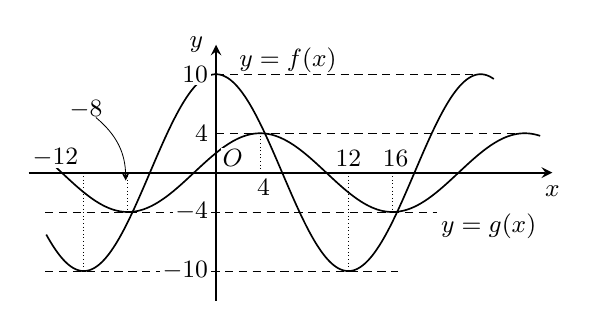
\begin{tikzpicture}[line width=0.6pt, x=0.14cm, y=0.125cm, >=stealth]
  \draw[densely dashed, line width=0.3pt] (0,10) -- (24,10);
  \draw[densely dashed, line width=0.3pt] (0,4) -- (28,4);
  \draw[densely dashed, line width=0.3pt] (-15.5,-4) -- (20,-4);
  \draw[densely dashed, line width=0.3pt] (-15.5,-10) -- (16.5,-10);
  \draw[densely dotted, line width=0.3pt] (-12,0) -- (-12,-10);
  \draw[densely dotted, line width=0.3pt] (-8,0) -- (-8,-4);
  \draw[densely dotted, line width=0.3pt] (4,0) -- (4,4);
  \draw[densely dotted, line width=0.3pt] (12,0) -- (12,-10);
  \draw[densely dotted, line width=0.3pt] (16,0) -- (16,-4);
  \draw[->, line width=0.7pt] (-17,0) -- (30.5,0) node[below=1pt, font=\small] {$x$};
  \draw[->, line width=0.7pt] (0,-13) -- (0,13) node[left=1pt, font=\small] {$y$};
  \draw[domain=-15.4:25.2, samples=240, smooth] plot (\x, {10*cos(15*\x)});
  \draw[domain=-14.6:29.4, samples=240, smooth] plot (\x, {4*cos(15*(\x-4))});
  \node[anchor=east, font=\small, fill=white, inner sep=1pt] at (-0.4,10) {$10$};
  \node[anchor=east, font=\small, fill=white, inner sep=1pt] at (-0.4,4) {$4$};
  \node[anchor=east, font=\small, fill=white, inner sep=1pt] at (-0.4,-4) {$-4$};
  \node[anchor=east, font=\small, fill=white, inner sep=1pt] at (-0.4,-10) {$-10$};
  \node[anchor=south east, font=\small, fill=white, inner sep=0.5pt] at (-12.3,0.4) {$-12$};
  \node[anchor=south west, font=\small, fill=white, inner sep=0.5pt] at (0.4,0.4) {$\pt{O}$};
  \node[anchor=north, font=\small, fill=white, inner sep=0.5pt] at (4.3,-0.5) {$4$};
  \node[anchor=south, font=\small, fill=white, inner sep=0.5pt] at (12,0.4) {$12$};
  \node[anchor=south, font=\small, fill=white, inner sep=0.5pt] at (16.3,0.4) {$16$};
  \node[font=\small] at (-11.8,6.4) {$-8$};
  \draw[->, line width=0.3pt] (-10.9,5.6) to[bend left=25] (-8.2,-0.8);
  \node[anchor=west, font=\small] at (1.2,11.4) {$y=f(x)$};
  \node[anchor=west, font=\small] at (19.5,-5.4) {$y=g(x)$};
\end{tikzpicture}
